\chapter{Agent}
\label{Agent}
In this chapter we are going to present the main function that are necessary for the agent in order to be functional in the field. Every part of agent's software will be extensively described.


\section{Agent Architecture}
\label{Architecture}
Before seeing each part of the agent software separately, it is time to describe the framework's architecture. Figure \ref{fig:Architecture}
shows this architecture. Soccer Simulation Server known as \textbf{rcssserver3d} is responsible for sending to the agent perception messages. Communication layer is the one that handles the connection between the agent and the server. In agent layer, these messages are handled by a string parser which is responsible for updating all agent's beliefs in structures. Consequently, functions that require new perceptions start. Find his location in the field or check if he is fallen on the ground are few of them. Behavior is a main part of every agent's process. Agent has to combine his knowledge and beliefs about the world state and act properly. Behavior is this function which takes as input the world state and gives agent an action to perform as output. In our approach, only goalkeeper ''runs'' an independent behavior, the other eight field players start a communication procedure in order to inform goalkeeper about their beliefs about the world state and some of their attributes. Goalkeeper is going to decide about the actions that every field player should do. So, we can realize that field players do not execute any behavior. We are going to describe coordination procedure later in a separate chapter.
Communication controller and motion controller are responsible for handling agent's requests for sending possible messages to his team mates or a movement that has to be executed. These two controllers send in every cycle if it is necessary effector messages to the connection layer which will send them back to soccer simulation server.\\
\begin{figure}[htb!]
\centering
  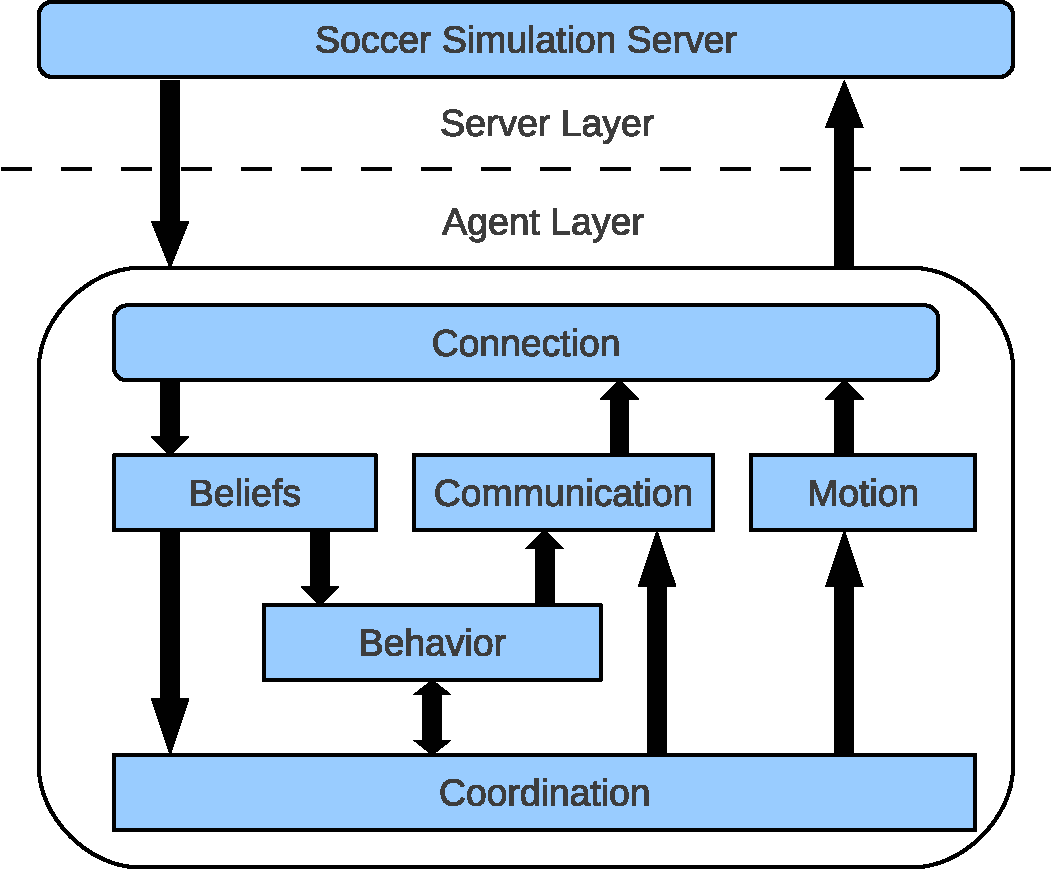
\includegraphics[scale=0.6]{Chapter3/figures/Arch.pdf}
  \caption{Agent's Architecture.}
  \label{fig:Architecture}
\end{figure}


\section{Connection}
The SimSpark server hosts the simulation process that manages the soccer simulation. It is responsible for advancing the game from on cycle to the next. So, each agent
connects to this server. Agents receives messages from the server in every 20ms; These messages includes information about all agent's perceptions. As we can see in the Figure \ref{fig:Simulation-Update-Loop}, SimSpark Server sends to each agent sense messages in the beginning of every cycle. Every agent who is willing to send an action message, he can send it in the end of this cycle, Server is going to receive at the same time it will send the next sense message.
\begin{figure}[htb!]
\centering
  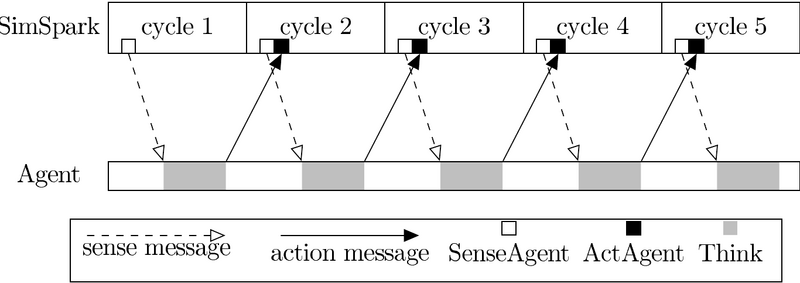
\includegraphics[scale=0.4]{Chapter2/figures/800px-SimulationUpdateLoopSynchronizationBetweenSimSparkAndAgent.png}
  \caption{Simulation Update Loop.}
  \label{fig:Simulation-Update-Loop}
\end{figure}



\section{Perceptions}
Perceptions in simulation soccer are quite different in comparison with real robots' competitions. We do not receive data from agent's sensors but from the server, which send them to us in every cycle. These messages have this form:\\
\begin{verbatim}
(time (now 46.20))(GS (t 0.00) (pm BeforeKickOff))(GYR (n torso)
(rt 0.00 0.00 0.00))(ACC (n torso) (a 0.00 -0.00 9.81))(HJ (n hj
1)(ax 0.00))(HJ (n hj2) (ax 0.01))(See (G2R (pol 14.83 -11.81 1.
08))(G1R (pol 14.54 -3.66 1.12)) (F1R (pol 15.36 19.12 -1.91))(F
2R (pol 17.07 -31.86 -1.83)) (B (pol 4.51 -26.40 -6.15)) (P (tea
m AST_3D)(id 8)(rlowerarm (pol 0.18 -35.78 -21.65)) (llowerarm (
pol 0.19 34.94-21.49)))(L (pol 8.01 -60.03 -3.87) (pol 6.42 51.1
90 -39.13 -5.17))(L (pol 5.91 -39.06 -5.11) (pol 6.28-29.26 -4.8
8)) (L (pol 6.28 29.34 -4.95)(pol 6.16 -19.05 -5.00)))(HJ(n raj1
) (ax -0.01))(HJ (n raj2) (ax -0.00))(HJ (n raj3)(ax -0.00))(HJ(
n raj4) (ax 0.00))(HJ (n laj1) (ax 0.01))(HJ (n laj2) (ax 0.00))
\end{verbatim}
The above message is just an example message our agent has been sent by simulation server
during game time. It includes information about the server time, the game state and time, the values of each one of his joints and data from vision, acceleration, gyroscope and force sensors. We parse this messages and saves data in appropriate for each type of perception data structures. Figure \ref{fig:BeliefsUpdate} illustrate this procedure.
\begin{figure}[htb!]
\centering
  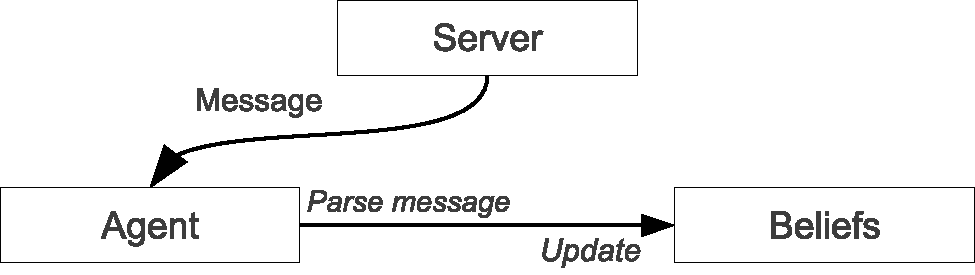
\includegraphics[scale=0.6]{Chapter3/figures/Message.pdf}
  \caption{Beliefs Update.} 
  \label{fig:BeliefsUpdate}
\end{figure}
\\


\section{Localization Process}
Once we have all the necessary beliefs updated, it is time for us to use them in order to locate our agent in the field. A brief description of the localization process follows.\\
\\
{\bf Localization Process} \cite{Localization}\\
\\
Localization process is executed every three cycles (60ms), every time that we have received observations from the vision perceptor. If we have visible objects in our field of view, we organize them in terms of their type. There are three types: Landmarks, Co-Players and Opponent Players. 

After organizing all visible objects, we only make use of the landmarks to find our position in the field. A key restrictive factor is that 
agents are only equipped with a restricted vision perceptor which limits the field of their view to 120 degrees. An example of this limitation is shown in the figure \ref{fig:fieldofview}. We could realize that localization process would have been more easier if there were a omni-directional field of view.
\begin{figure}[htb!]
\centering
  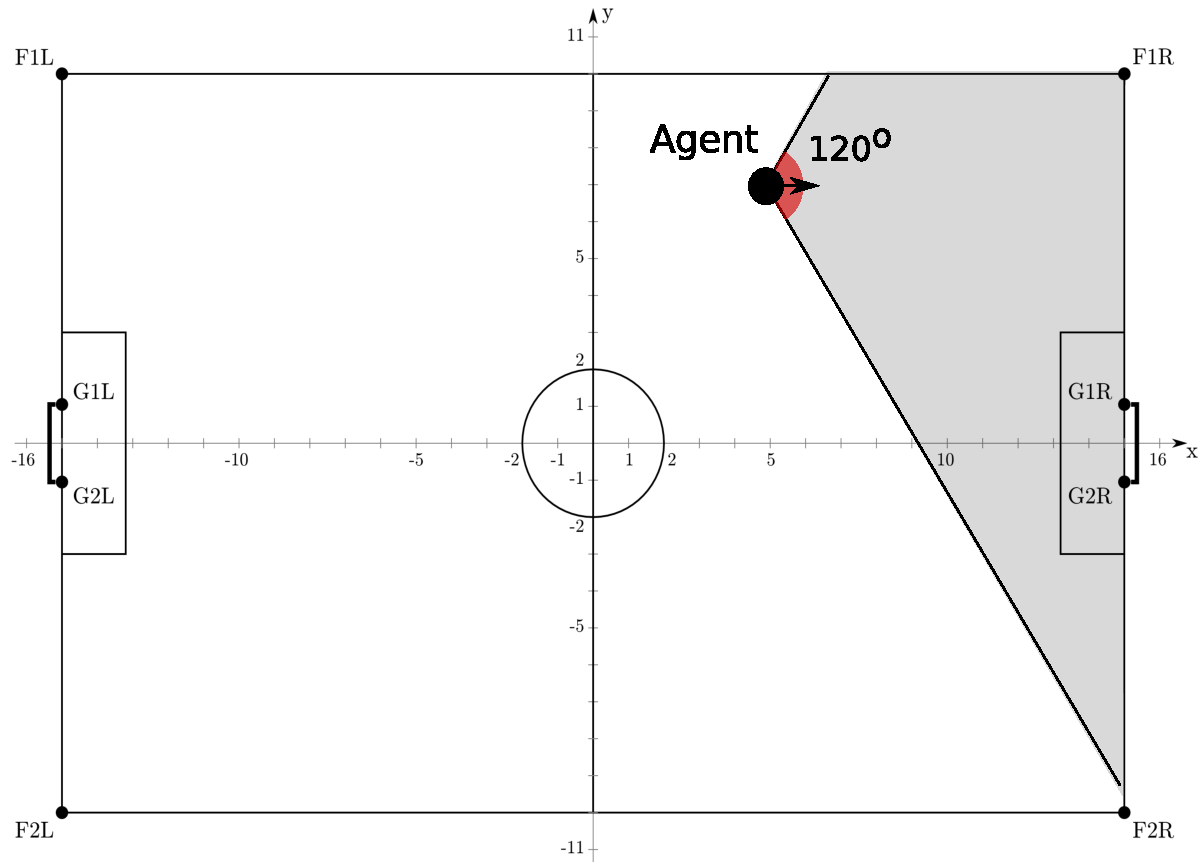
\includegraphics[width=0.8\textwidth]{Chapter3/figures/LViewAngle.pdf}
  \caption{Nao's Field of View.} 
  \label{fig:fieldofview}
\end{figure}
 
Localization process became possible through three main functions. The first function, takes two landmarks as arguments and returns to us a possible position for our agent. If our agent sees more than two landmarks, then this function is called for every combination of two landmarks and in the end we compute the average position of these results. If our agent sees less than two landmarks, then he has a complete unawareness of his position in the soccer field. Figure \ref{fig:Localization} shows how this function works. For every two landmarks there are two circles with radius as the distance we see each of them. These two circles intersect at 2 points. We keep as a final result the point which is within field's limits, rejecting the other.
\begin{figure}[htb!]
\centering
  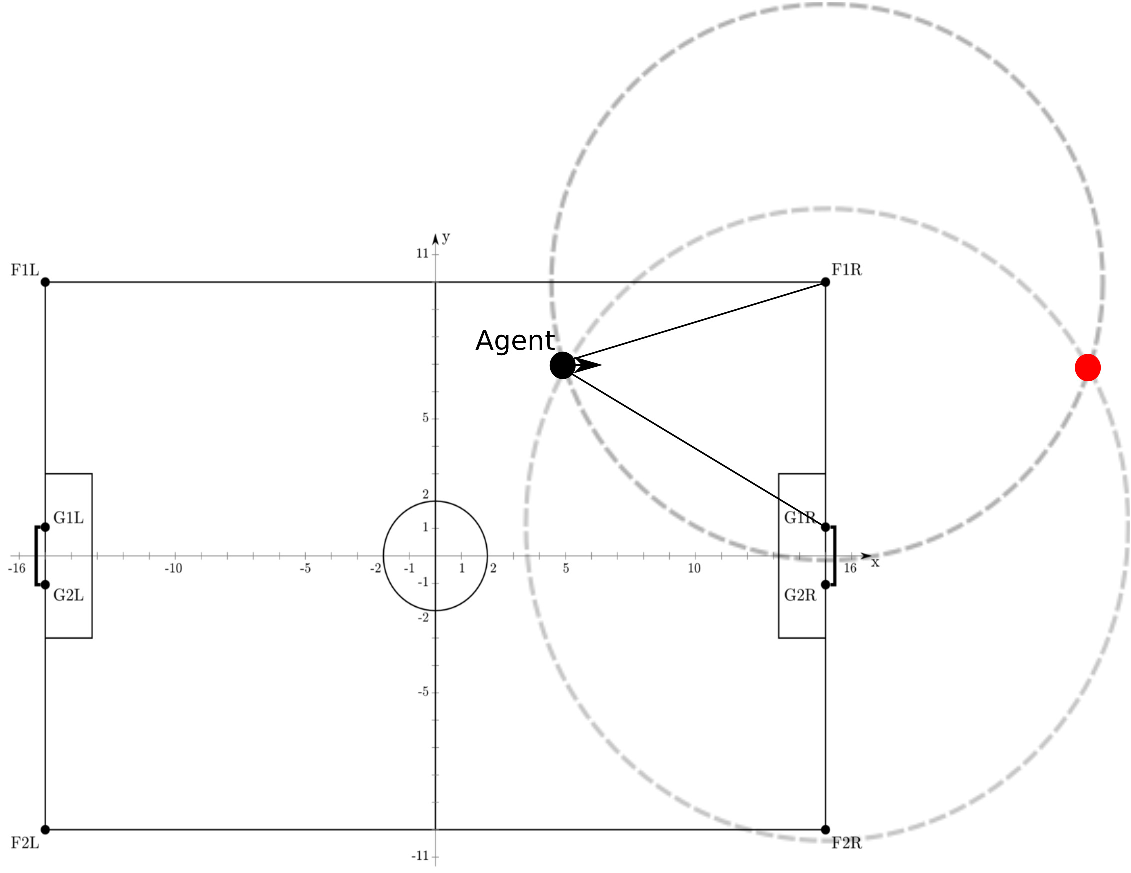
\includegraphics[width=0.8\textwidth]{Chapter3/figures/Localization.pdf}
  \caption{Localization Main Idea.} 
  \label{fig:Localization}
\end{figure}

Except from the calculation of our position in the soccer field, localization is responsible to locate ball and other agents in the field as well. Knowing our position helps us locate other objects too. For every other object which is locates in our field of view, vision perceptor informs us about its vertical angle, its horizontal angle and its distance from our agent. This information is enough for the calculation of their exact positions. Finally, after the localization process end, we are able to have the following observations:\\

\begin{description}
	\item[Our Position] Only if agent sees more than one landmarks.
	\item[Body Angle] Only if agent knows his position.
	\item[Other Agents Positions]	Only if agent knows his position and other agents are located in the field of his view.
	\item[Ball Position] Only if agent knows his position and ball is located in the field of his view.
\end{description}
In Figure \ref{fig:LocalizationResults} we can see the results which are given by the localization process.
\begin{figure}[htb!]
\centering
  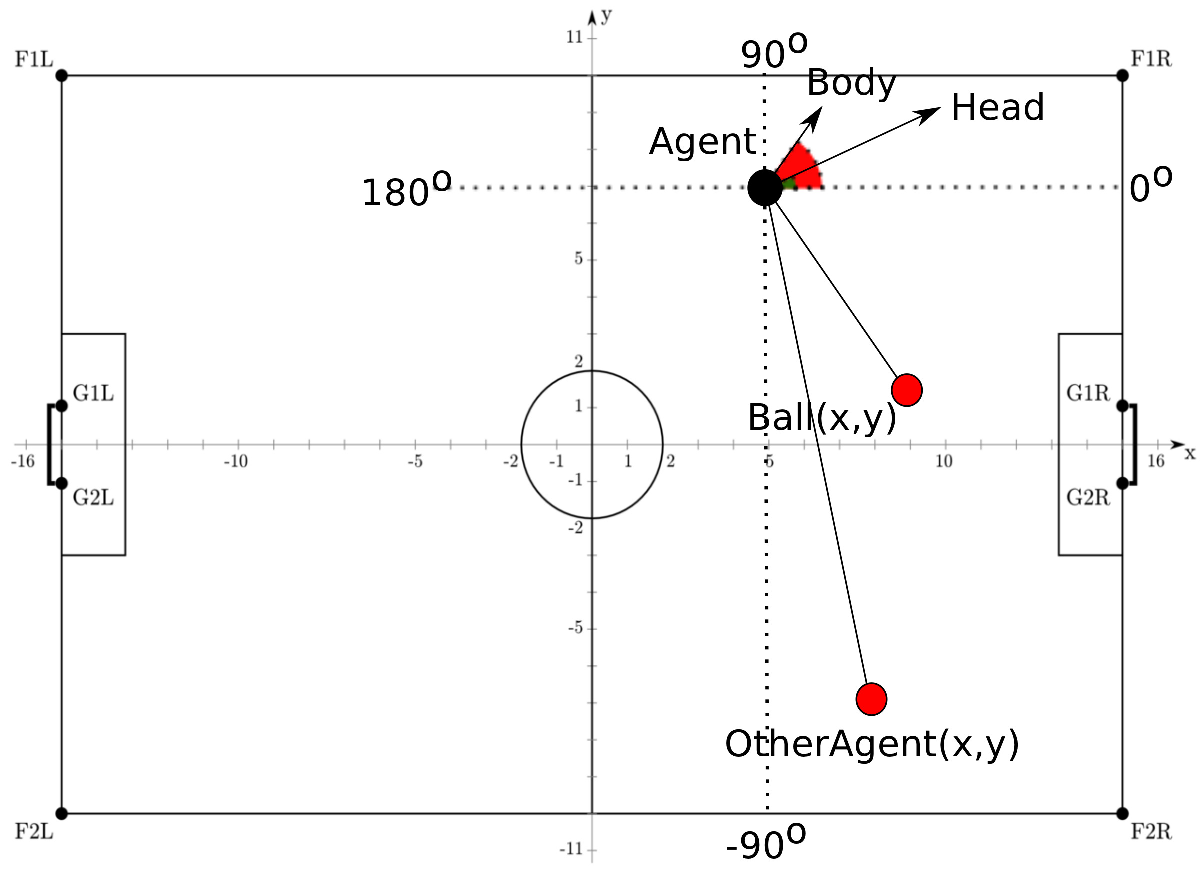
\includegraphics[width=0.8\textwidth]{Chapter3/figures/LocalizationResults.pdf}
  \caption{Localization Results.} 
  \label{fig:LocalizationResults}
\end{figure}
\hfill









\section{Localization Filtering}
In absence of a stochastic localization system, we are forced to ensure that localization results are qualitative enough for us to rely on. Due to the symmetry of the field's landmarks and faulty observations due to noise existence, localization is not always accurate enough to depend on. Therefore, a kind of filtering is required for  observations are taken by the localization process.
\begin{algorithm}[ht!]
\caption{Localization Filtering}
\label{LocalizationFiltering}
\begin{algorithmic}[1]
\STATE {\bf Input: }$Observation$
\STATE {\bf Output: }$FilteredPosition$
\IF{$size(Queue) = 0$}
\STATE $Queue.Add(Observation)$
\STATE $MyPosition = AVG(Queue)$
\ELSIF{$size(Queue) < MaxSize$}
\IF{$Observation \not\approx AVG(Queue)$}
\STATE $Queue.Remove()$
\ELSE
\STATE $Queue.Add(Observation)$
\STATE $MyPosition = AVG(Queue)$
\ENDIF
\ELSE
\IF{$Observation \not\approx AVG(Queue)$}
\STATE $Queue.Remove()$
\ELSE
\STATE $Queue.Remove()$
\STATE $Queue.Add(Observation)$
\STATE $MyPosition = AVG(Queue)$
\ENDIF
\ENDIF
\end{algorithmic}
\end{algorithm}
Algorithm \ref{LocalizationFiltering} describes the process of localization filtering. In general, localization process provides agents with not consecutive faulty observations. The general idea that we follow in our approach is that agents take one thousand observations per minute. Therefore, it will be easy for them not to take into consideration the observations with the biggest fault. To overcome this difficulty, we came up with a simple and clever approach. The average of a queue full of observations always gives us our agent's position in the field. When an observation is coming, we check if the queue is empty or full; If it is empty, we just add the observation into the queue. If it is full of elements, then we check if the new observation seems faulty in comparison to the average of the queue. If it does, we do not take it into account and we just remove an element from the queue. If not, then we add it to the queue.
If queue is neither empty nor full, we make the same procedure checking if it is a faulty observation, with the only difference that we do not remove any element if it is not. Localization filtering applies for both the calculation of our agent's position and the ball's position. Its result was the improvement of the localization results in an adequate degree in order to rely on them with confidence. This filtering smooths the belief of our belief's position and rejects every faulty observation.


%%%%%%%
\section{Motions and Movement}
\label{Motions}
In robotics, we could define a motion as a sequence of joint poses. A pose is a set of values for every joint in the robot's body at a given time.
For example, for a given set of n-joints a pose could be defined as:\\
\begin{center}
$Pose(t)$=$\lbrace J_{1}(t),J_{2}(t),...,J_{n}(t) \rbrace$\\
\end{center}
\begin{figure}[htb!]
\centering
  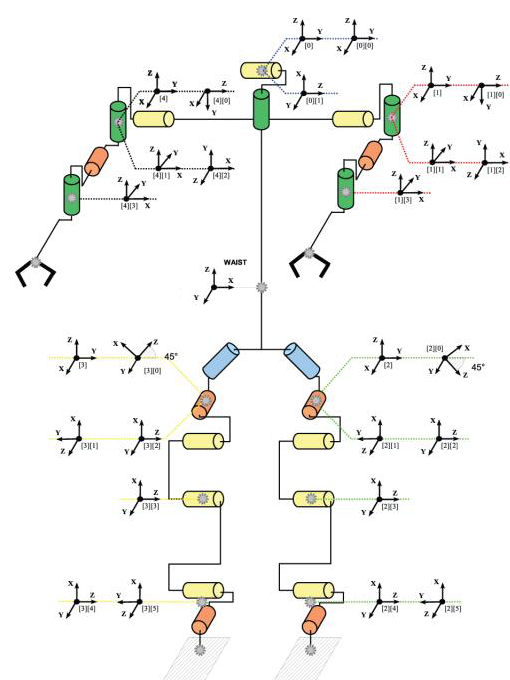
\includegraphics[width=0.3\textwidth]{Chapter3/figures/Models_NaoAnatomy.png}
  \caption{Nao's anatomy.}
  \label{fig:NaoAnatomy}
\end{figure}
Simulated Nao has 22 degrees of freedom. That practically means that it has 22 hinge joints.
Figure \ref{fig:NaoAnatomy} shows Nao's anatomy.
Motions are very important part of every team taking part in the simulation league. Most of the teams in this league make use of dynamic movement which is a major advantage for their side. In this approach, we are using motion files. Motion files are set of poses which has static and standard values for each joint in every type of movement. The difference between static motion files and dynamic movement is that dynamic movement takes into consideration the center of the body's mass and the direction in which we want to head the agent. This movement gives robot better body balance and fast movement especially in situations when robot wants to change direction or to make a turn. In this approach we are using two kinds of static motion files. Text based and XML based motion files. Agent, before initializes himself in the field read these motion files and saves them into the dynamic memory to be ready to use them without any need of reading them every time he needs them.


\subsection{XML-File Based Motions}
These motion files has been created from FIIT RoboCup 3D project. They have XML structure and it was easy for us to implement them into our project. Structure of these xml motion files is shown below.
\begin{verbatim}

		<phase name="Start" next="Phase1">
			<effectors>
				Joint Values
			</effectors>
			<duration>duration</duration>
		</phase>
		<phase name="Phase1" next="Phase2">
			<effectors>
				Joint Values
			</effectors>
			<duration>duration</duration>
		</phase>
		<phase name="Phase2"next="Phase1">
			<effectors>
				Joint Values
			</effectors>
			<duration>duration</duration>
			<finalize>Final</finalize>
		</phase>
		<phase name="Final">
			<effectors>
				Joint Values
			</effectors>
			<duration>duration</duration>
		</phase>

\end{verbatim}
It is easy to understand that each movement is split into phases. Each phase has a duration and values for every necessary for the movement joint of the robot. Moreover, every phase has an index which points to the next phase. For example, we can see that the first phase ''Start'' has an index for the next phase: ''Phase1''. Phases with a finalize field help us to end each movement. For example, the phase:''Phase2'' has a finalize index which points to the phase: ''Final'', this means that if we want to end this type of movement, we have to continue with the execution of the finalize phase and not with the next.
\subsection{XML-File Based Motion Controller}
Motion controller is a major part of movement ability of the robot. It is responsible for handling the movement requests by the agent. Agent has not access in motion controller himself but he has access in the motion trigger. We could imagine this trigger as a variable which can only be changed by the agent. Each agent declares the movement he is willing to perform in this variable.
Motion controller reads this variable in every cycle and generates an hinge joint effector string which is the result of this process.
\begin{figure}[htb!]
\centering
  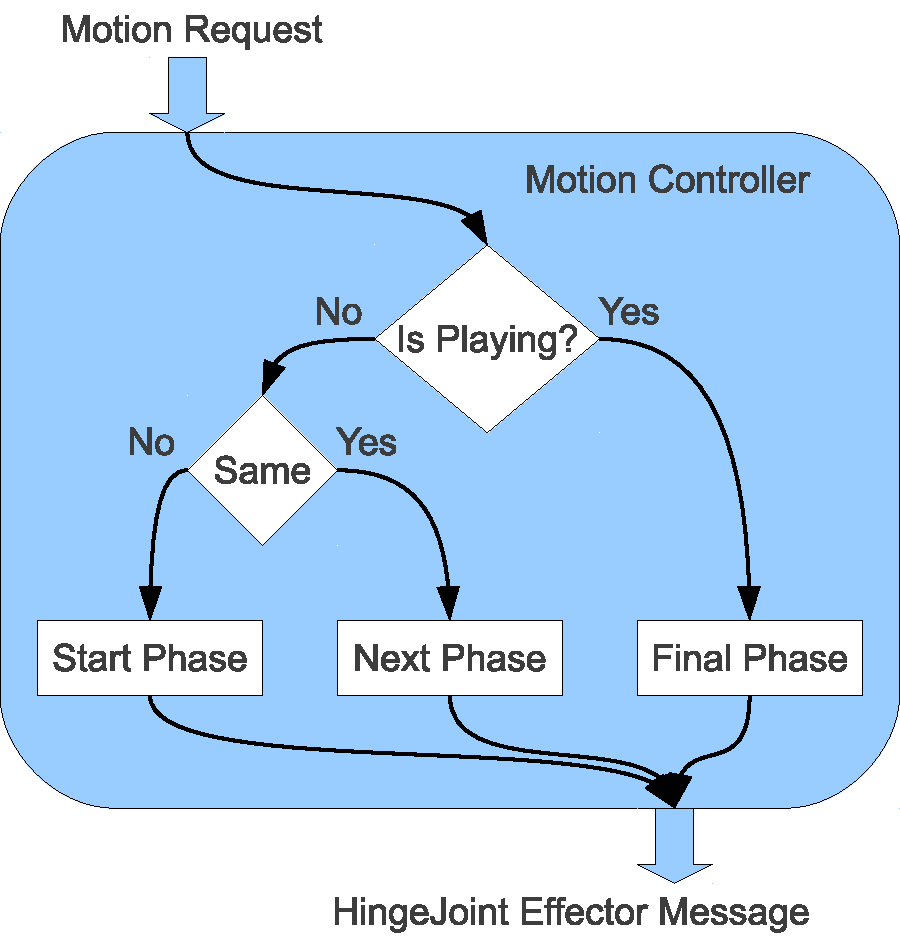
\includegraphics[scale=0.6]{Chapter3/figures/MotionController.pdf}
  \caption{Motion Controller.}
  \label{fig:MotionController}
\end{figure}


In Figure \ref{fig:MotionController} we show the general architecture of the motion controller. Motion controller checks if there is a motion which is playing already. If yes, motion controller tries to finalize the playing movement in order to start playing the new requested movement.
\begin{figure}[htb!]
\centering
  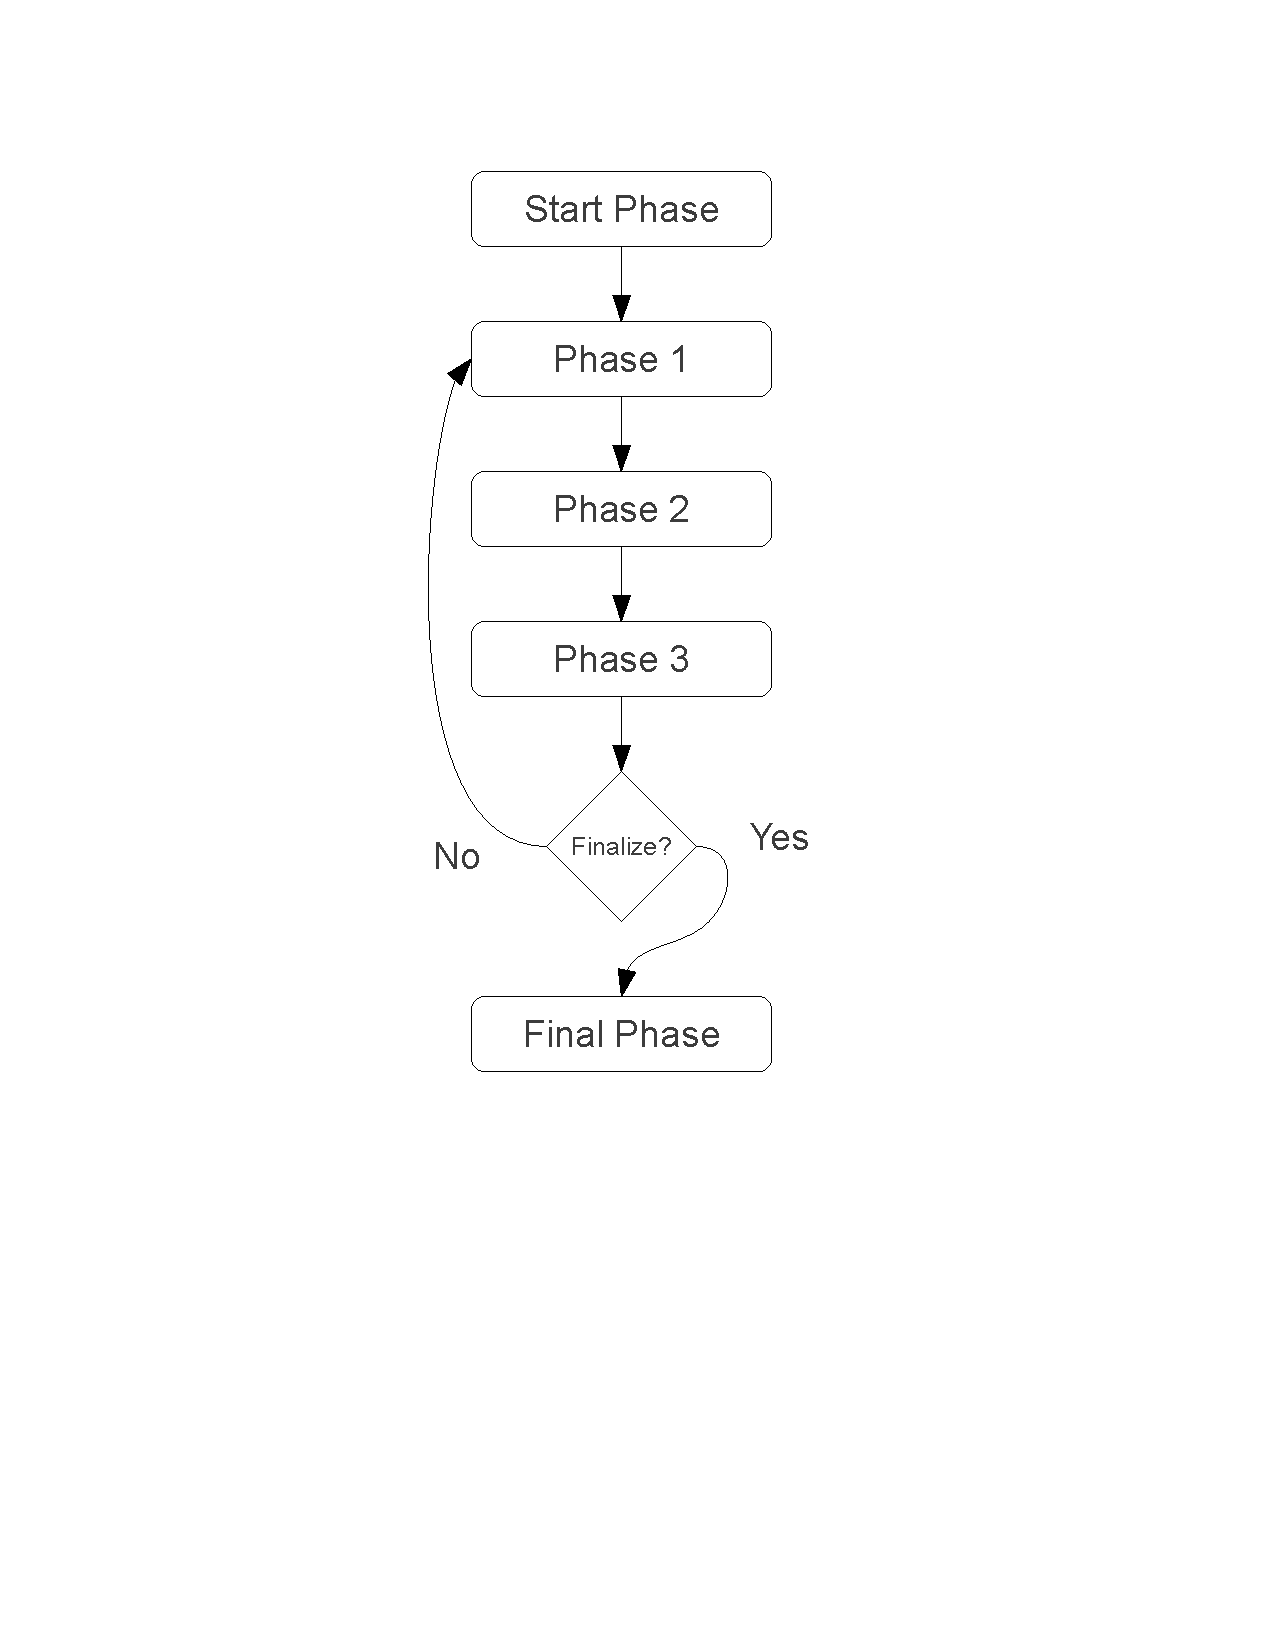
\includegraphics[scale=0.6]{Chapter3/figures/MotionSequence.pdf}
  \caption{Phase Sequence.}
  \label{fig:PhaseSequence}
\end{figure}


Figure \ref{fig:PhaseSequence} describes the exact motion sequence. In general, XML motions is created to include cycles. For example, walking motion has three main phases which create a cycle. If motion trigger has not changed at the last phase, we have to continue with the execution of the first phase not with the final one. As we saw in the structure of every XML based motion file, each phase has a set of joint values. These values are in degrees scale. To generate motions for our agent we need to create a motion string. This string holds information about the velocity we want to give in every joint involved in each motion phase. This velocity can be calculated by:
\begin{center}
$Desired Velocity$ = $Already Joint Value$ - $Desired Joint Value$
\end{center}
This is the desired velocity of every joint. Furthermore, every phase has a duration in which has to be executed. So, phase duration has to be divide with the duration of every server cycle. This will give us the number of cycles this phase will be performed by the agent.
\begin{center}
$Cycles Number = \frac {Phase Duration} {Cycle Duration}$
\end{center}
Now, we have each joint's velocity and the duration in cycles. We can calculate, how much will be the speed of every joint in order to reach to the desired joint value in this time limit.
\begin{center}
$Velocity = \frac {Desired Velocity} {Cycles Number \ast CycleDuration} $ Degrees/Sec
\end{center}
This velocity is calculated for every involved joint in the motion. The final output of the motion controller will be send to the server.


%%%%%%%%%%%
\subsection{Text-File Based Motions}
The other kind of motion files we are using is created by Webots simulator. These text based motion files have simpler structure than the XML motion files. In default, each pose lasts for two simulation cycles (40ms). Structure of these xml motion files is shown below.
\begin{verbatim}
#WEBOTS_MOTION,V1.0
LHipYawPitch,LHipRoll,LHipPitch,LKneePitch,LAnklePitch,...
00:00:000,Pose1,0,-0.012,-0.525,1.05,-0.525,0.012,0,...
00:00:040,Pose2,0,-0.011,-0.525,1.05,-0.525,0.011,0,...
00:00:080,Pose3,0,-0.009,-0.525,1.05,-0.525,0.009,0,...
00:00:120,Pose4,0,-0.007,-0.525,1.05,-0.525,0.007,0,...
00:00:160,Pose5,0,-0.004,-0.525,1.05,-0.525,0.004,0,...
00:00:200,Pose6,0,0.001,-0.525,1.051,-0.525,-0.001,0,...
00:00:240,Pose7,0,0.006,-0.525,1.05,-0.525,-0.006,0,...
00:00:280,Pose8,0,0.012,-0.525,1.05,-0.525,-0.012,0,...
00:00:320,Pose9,0,0.024,-0.525,1.05,-0.525,-0.024,0,...
\end{verbatim}
At the second row, there are the definition for all joints which are related to the specific movement. For example, walking motion requires only the joints from both robot's legs. The next rows from left to right have information for the duration of each pose, the pose name and finally the joints' values for each joint in radian scale in the same order as they are defined in the second row.


\subsection{Text-File Based Motion Controller}
Motion controller for text based motions is based on the same principle as the XML controller. The joint values in the motion files represent radians. So, we convert these values into degrees and then we proceed with the next steps. Each pose lasts for one or two cycles depending on the speed we want each motion to be executed. This motion controller could be customized easily to perform motions differently. There are parameters that can be changed such as:
\begin{description}
	\item[Speed] How many cycles from pose to pose.
	\item[Speed Control] How fast we want pose to be executed.
	\item[Pose Offset] Pose Offset = 2, we execute pose1,pose3,pose5,...
	\item[Hardness Factor]	Hardness Factor = 0.9, we multiply the velocity with this factor.
\end{description}
The velocity of every joint is calculated by:\\
\\
$Desired Velocity$ = $Already Joint Value$ - $RadiansToDegrees(Desired Joint Value)$
\\
\\
$Velocity = \frac {Desired Velocity \ast Hardness Factor} {Duration
 \ast CycleDuration} Degrees/Second$\\
\\
This velocity is calculated for every involved joint in the motion. The final output of the motion controller will be send to the server.

\subsection{Dynamic Elements in Movement}
In contrast with the general idea about static motion files stated in the beginning of this Section \ref{Motions}, we have tried to implement some dynamic features in our movements. There is not so much room for improvement in these static motions but we achieved to have nice results.
\begin{description}
	\item[Walk Leaning] Walking can be lean to the right and to the left. There was an improvement on overall performance as agent should turn his body every in every occasion.
	\item[Walk Slowdown] Its important our agent to slowdown his speed in order to stop his body with more stability.
	\item[Turn]	Agents turns his body as much as he needs from 7 to 40 degrees. Figure \ref{fig:Turn} shows this process. X-axis is the hardness factor and Y-axis presents how much each motion turns the body of the agent in degrees.
\end{description} 
\begin{figure}[htb!]
\centering
  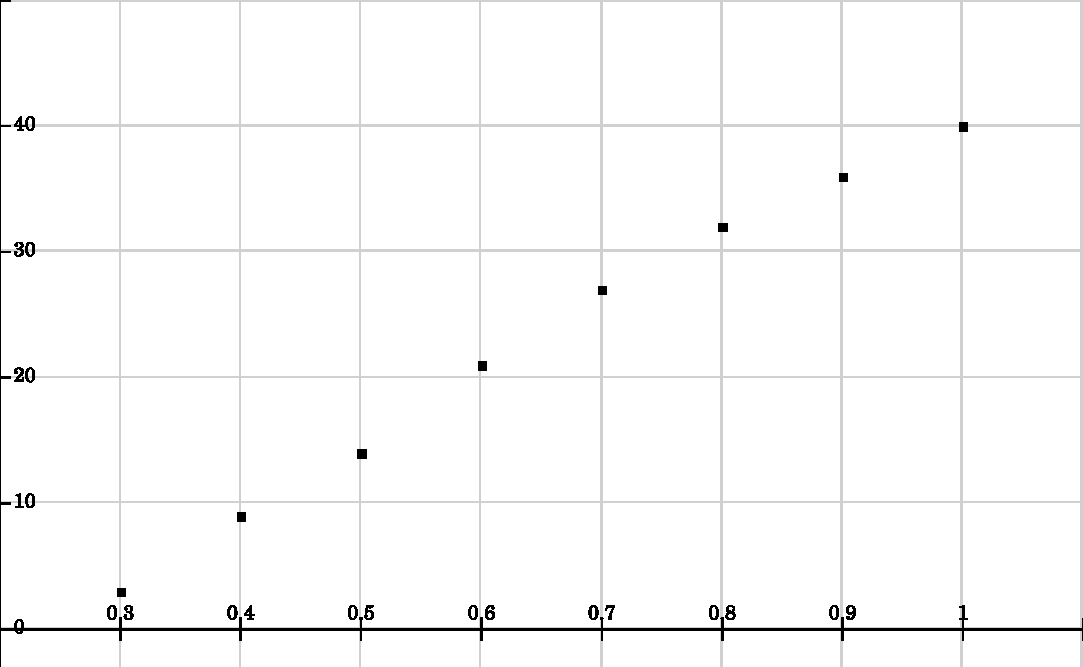
\includegraphics[width=0.8\textwidth]{Chapter3/figures/DynamicTurn.pdf}
  \caption{Dynamic Turn.}
  \label{fig:Turn}
\end{figure}


\section{Actions}
In this section, we describe the way that agent can affect and change his environment. In general, actions are the results of the agent's perception in combination with his procedure of thinking.
In our approach actions are split into groups in terms of their complexity and their type.

\subsection{Simple}
Simple actions make use only of movements and have a simple structure. These simple actions are:
\begin{description}
 \item[Turn To See Ball] This action results in turning the agent until ball is in his field of view. In this action we take observations from vision perceptor in order to locate ball.
 
 \item[Turn To Ball] This action turns agent towards the direction of the ball.
 
 \item[Turn To Locate] This is the default action each agent does when he loses his position ( sees less than two landmarks ) in the field. It helps agent to relocate itself in the field.
 
 \item[Walk To Ball] Agent walks towards the ball. He stops when the ball is close enough for him to shoot it. Remind, that distance from ball comes from vision perceptor and defines the distance between the agent's vision perceptor - which is attached to agent's head, and the ball. So, it is better for agent to calculate the distance between his feet and the ball. This became feasible thought direct kinematics via trigonometry in 2-dimension space. Starting from agent's ankle(0,0) it is easy to calculate every joint's position in 2D-space from ankle to head. Figure \ref{fig:2dkinematics} shows how joint values are related with the feet's distance from the ball.
 
 \begin{figure}[!h]
\centering
  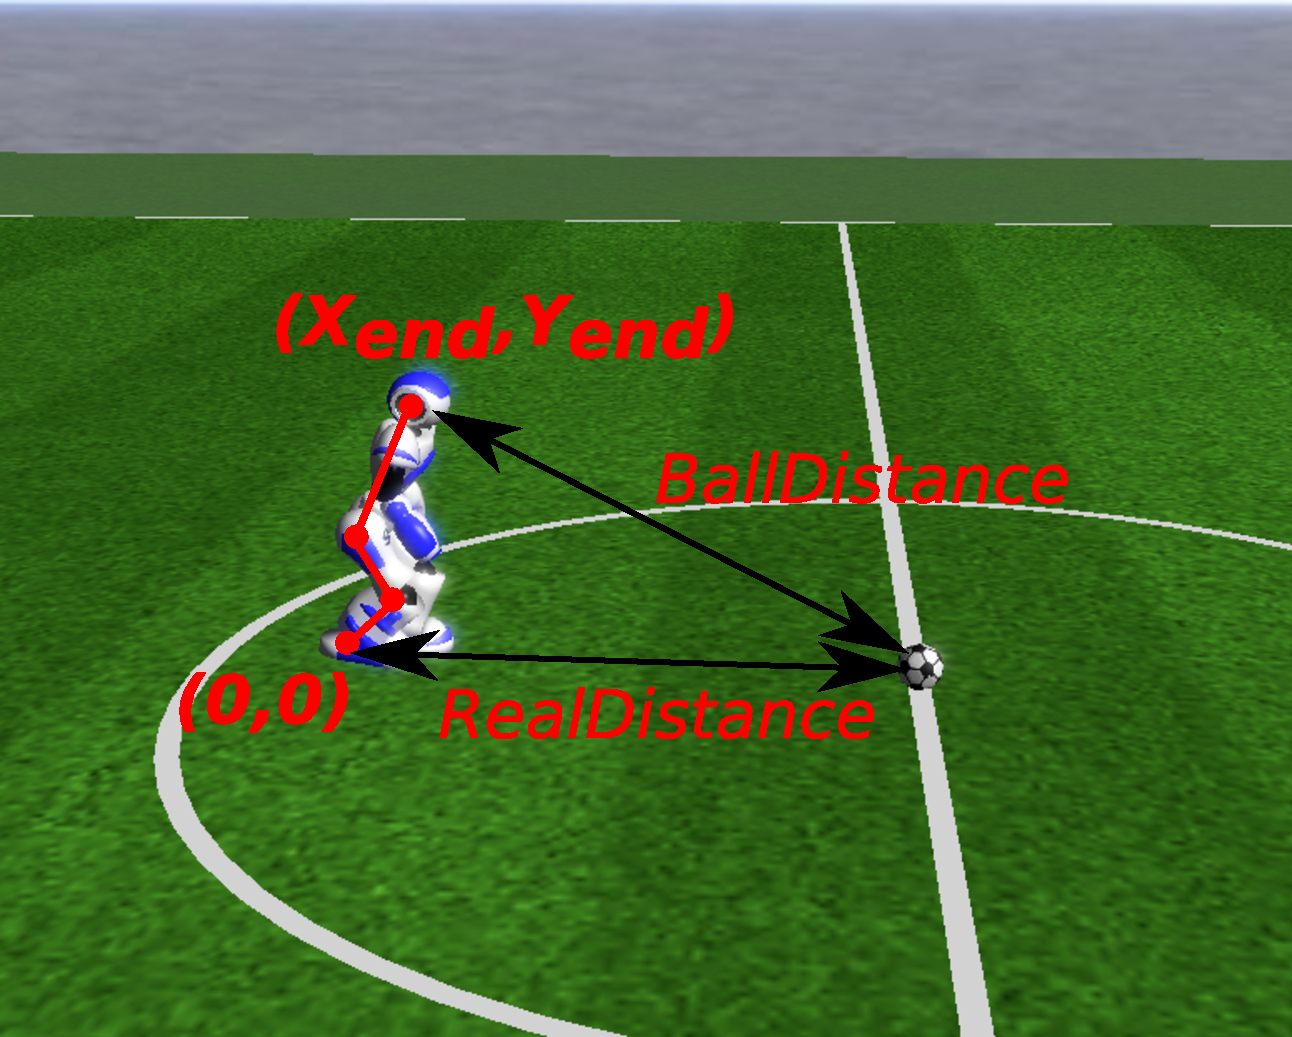
\includegraphics[trim=0cm 4cm 0cm 4cm, clip,width=0.8\textwidth]{Chapter3/figures/2dkinematics.pdf}
  \caption{Ball Distance from Agent's Feet.}
  \label{fig:2dkinematics}
\end{figure}
 \item[Stand Up] Agent executes it when he is fallen on the ground in order to get up.
 \item[Prepare Kick] Agent executes it before performs a kick. This action is needed in order to have a proper position to kick ball successfully. Figure \ref{fig:NaoKick} shows an example in which we are showing the agent's position before the kick.
  \begin{figure}[!h]
\centering
  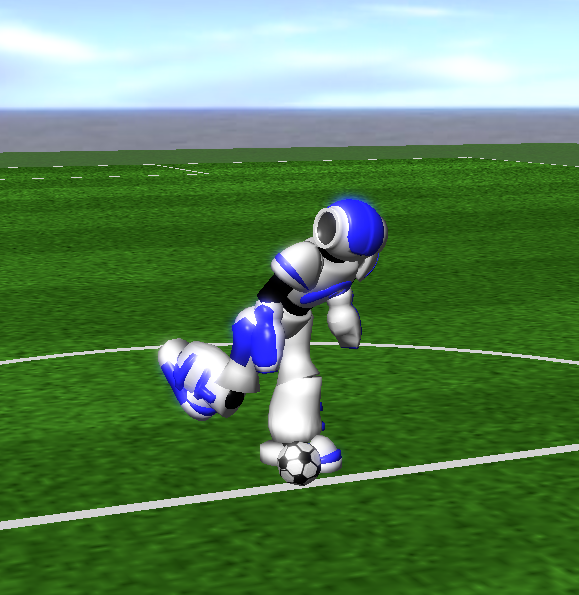
\includegraphics[trim=0cm 3cm 0cm 4cm, clip,width=0.6\textwidth]{Chapter3/figures/NaoKick.png}
  \caption{Nao Before Kick Ball.}
  \label{fig:NaoKick}
\end{figure}
\end{description}

\subsection{Complex}
Complex actions are created to make use of more than one simple actions and motions, they have a more complicated structure. These complex actions are:
\begin{description}
 \item[On Ball Action] This action uses Walk To Ball in order the agent to reach the ball. In this action we use the agent's belief about his location in the field to help us find the direction and the kick's type. This action has a finite state machine logic. Figure \ref{fig:GoKickBallToGoal} shows in what order this action is executed. In every state it is possible an opponent agent takes the ball away from agent. In this situation agent return to the initial state.
 \begin{figure}[!h]
\centering
  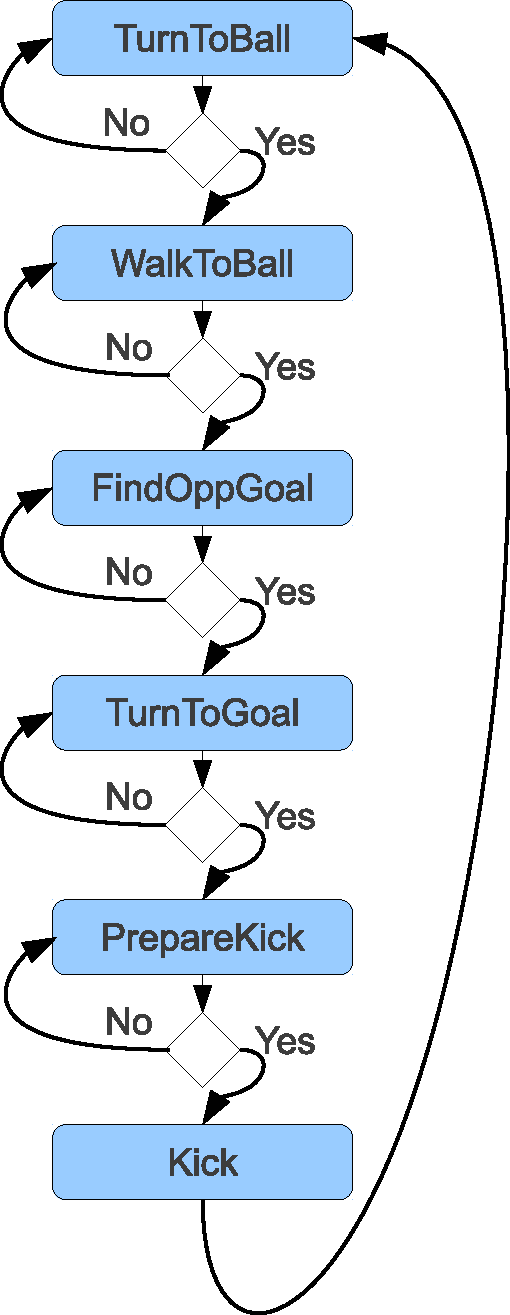
\includegraphics[width=0.25\textwidth]{Chapter3/figures/KickFSM.pdf}
  \caption{On Ball Action Logic Sequence.}
  \label{fig:GoKickBallToGoal}
\end{figure}
 \item[Walk To Coordinate]
 This action leads agent to a specific coordinate(x,y,theta) in the soccer field. To achieve this action we need to know our position in the field and the target coordinate. Agent is able to know his position so it is easy for us to calculate in which direction agent has to walk in order to get in the specific coordinate. Figure \ref{fig:WalkToCoordinate} shows in what direction agent should walk from the point $(X_{start},Y_{start})$, to the point $(X_{target},Y_{target})$. It is easy to find $\vartheta_{target}^{\circ}$:\\
\begin{center}
$d_{X} = X_{target} - X_{start}$\\
$d_{Y} = Y_{target} - Y_{start}$\\
$\vartheta_{target}^{\circ} = atan2(d_{X},d_{Y})$\\
$d_{target} = \sqrt{d_{X}^2 + d_{Y}^2}$
\end{center}

Been helped from the above calculations agent is always aware of the distance and the direction he has to travel towards his target position. 
 \begin{figure}[!h]
\centering
  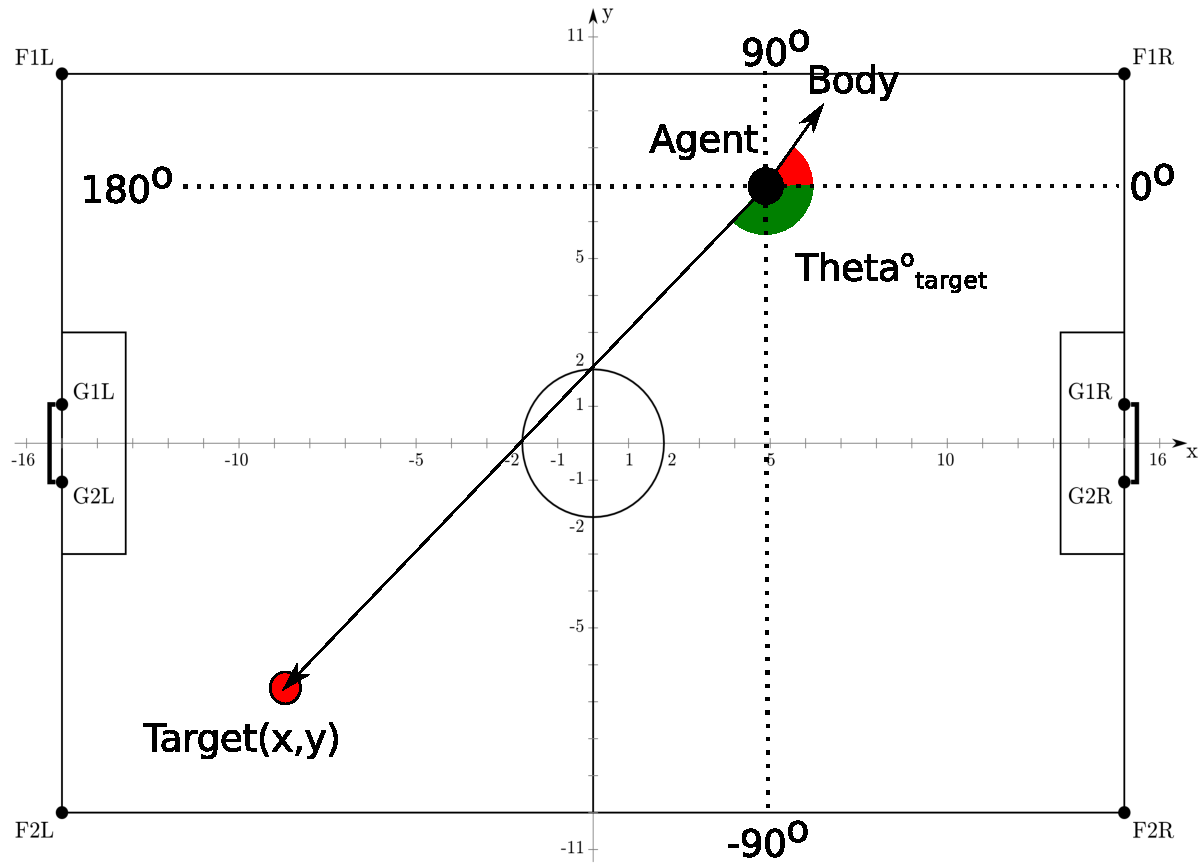
\includegraphics[width=0.8\textwidth]{Chapter3/figures/GoToPos.pdf}
  \caption{Walk To Coordinate Action.}
  \label{fig:WalkToCoordinate}
\end{figure}
 \item[Walk To Direction]
 This action leads agent to walk towards a specific direction.
 \item[Walk With Ball To Direction]
 As far as agent reaches the ball, he will try to keep the ball in front of him and walk towards a direction keeping into mind that the ball has to be always in front. This action is not yet functional in our approach as movements based on motion files make it hard for us keeping ball in front of our agent all the time.
\end{description}

\subsection{Vision}
Vision related actions are created to control the vision perceptor which is attached to the robot's head as well as to collect data from it in order to execute related actions such as obstacle avoidance. These vision related actions are:
\begin{description}
 \item[Head Movement] This action is related with the movement of the head in different occasions. Nao robot has two joints attached in the neck which give us the freedom of moving the head in relation to the action is being performed.
 \begin{description}
 \item[type 1] Head moves to its original position. Both joint-axis are given 0 degrees as desired angle.
 \item[type 2] Head moves until agent see the ball.
 \item[type 3] Head moves in relation to the ball's movement. In this type head follows the ball movement in condition that head does not exceed both axis thresholds.
 \item[type 4] Head make a harmonic movement in order agent to have a nice perception of his environment. This type used in obstacle avoidance action.
 \item[type 5] Head moves until agent can localize himself in the field.
 \end{description}
 \item[Watch Object Movement] This action requires that object is in agent's field of view. Knowing the direction and the speed of the moving object is only feasible if we keep in memory a short number of observations. We keep two sets of five observations which we have taken within a time offset. Finding the average position of each set gives a distance between these two positions. If this distance will be divided with the time difference of the two observation sets we are going to have the direction and the speed of the moving object.
 \item[Find Opponents Goal] This action is used in On Ball action in order to take observations about the direction of the opponents goal in relation to agent's body angle.
 \item[Percept Obstacles]
 An action that has the responsibility of having a good view of all obstacles which are located in agent's close range. Due to the fact that simulated Nao's head can move in horizontal axis from $120^{\circ}$ to $-120^{\circ}$ and our field of view is $120^{\circ}$ means that we can have a complete imaging from all obstacles which are located close to our agent.
So, in every cycle of Nao's head we store all obstacles in an array. It is usual to observe the same obstacle more than once, in this situation we compute the average of these observations. At the end of head's cycle we call the main action which tries to find alternative routes if there is an obstacle in our way.
 \item[Obstacle Avoidance]
 In a dynamic and a multi-agent environment like simulation soccer this action is more than necessary. However, there are some teams in simulated soccer competition which have not develop an obstacle avoidance system yet. In our framework there is a
 reliable and a well-tested system to avoid possible collisions with other agents as well as landmarks(only goal-posts).
  \begin{figure}[!h]
\centering
  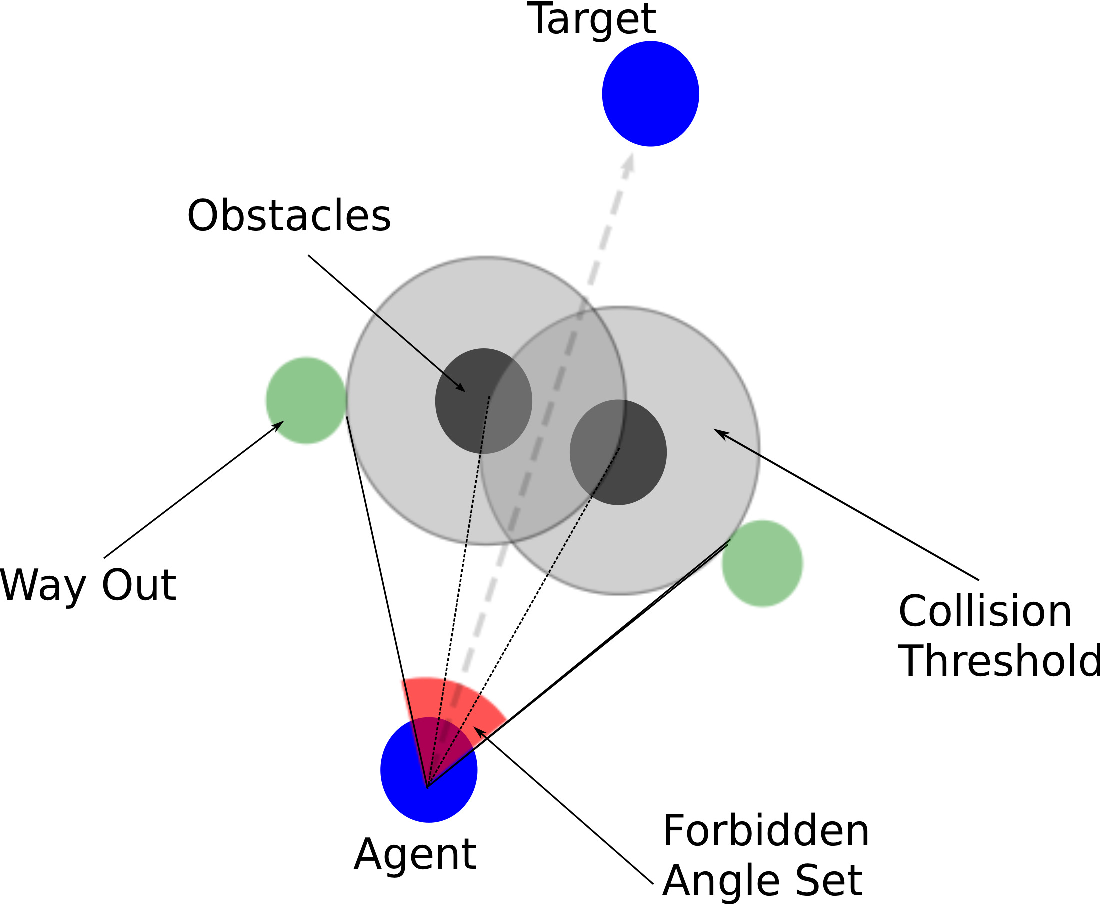
\includegraphics[width=0.6\textwidth]{Chapter3/figures/ObstacleAvoidance.pdf}
  \caption{Obstacle Avoidance.}
  \label{fig:ObstacleAvoidance}
\end{figure} 
\end{description}

Figure \ref{fig:ObstacleAvoidance} shows an example in which there are two obstacles between the agent and his target. During his walk to coordinate action agent scans the field for possible obstacles through the action mentioned above. If agent realizes that there is an object which blocks his way to the target in the same simulation cycle he starts computing the possible way out angles that he can choose in relation to his observations about all obstacles. For every obstacle, we calculate a set of two angles. These angles is determined by the distance between our agent and the obstacle and they imply in which direction we can avoid this obstacle. When these angles are calculated, we check every angle of each set if it belongs to another angle set as well. Angles which belong to another set are removed from the final list.
\begin{algorithm}[htb!]
\caption{Way Out Angle Set Computation}
\label{AngleSet}
\begin{algorithmic}[1]
\STATE {\bf Input: }$Obstacles = \lbrace O_{1},O_{2},...,O_{n} \rbrace $
\STATE {\bf Output: }$WayOutSet[ ]$
\FOR{{\bf each} i in Obstacles}
\STATE $WayOutSet.Add(Calculate(O_{a},t)),\vee t \in \lbrace right,left \rbrace$
\ENDFOR
\FOR{{\bf each} j in WayOutSet}
\FOR{{\bf each} t in $\lbrace right, left \rbrace$}
\IF{$WayOutSet_{j,t} \in WayOutSet_{k}, \vee k \in \lbrace 1,2 \ast n \rbrace , k \neq j$}
\STATE $WayOutSet.Remove(j,t)$
\ENDIF
\ENDFOR
\ENDFOR
\end{algorithmic}
\end{algorithm}

This process' algorithm is described in Algorithm \ref{AngleSet}. Once we have all the qualified angle sets from the algorithm, it is time to find coordinates which are safe in order to avoid the one or more obstacles. For each angle in these sets we calculate a specific coordinate. These coordinates in the soccer field will give us routes that are safe to follow. Now, we are going to calculate the cost for each route in respect with our body angle and the distance we have to travel to target if we follow this route. The route with the minimum cost is qualified to be followed by the agent. Calculating this cost will give as dynamically consistent results. If cost function outputs a specific route at time T, assuming that obstacles are not moving, this function will output the same route for every time t $>$ T, until we will have a clear of obstacles route to our target position.


\subsection{Other Sensors}

Other Sensors related actions are created to collect data from gyroscope, accelerometer and force resistance perceptors. In this category there is only one action. This action is called {\bf Check If Fall} and is responsible to check if our agent is fallen on the ground. In a multi-agent environment like SimSpark soccer simulator we should be aware about possible collisions with other agents or falls because the instability of movements. First of all, incoming perceptual inputs related to both gyroscope and accelerometer values are used to detect whether the robot has become subject of a turmoil. Taking values above a specific threshold from these two perceptors, it is possible that the robot has fallen, but we are not completely sure to perform a stand up action yet. It is not unusual to receive values above threshold due to a collision without a fall. So, we have to check the force resistance perceptors which are located on the sole of agent's feet. If these perceptors imply that the legs do not touch the ground then we are pretty sure to perform a stand up action.Foot pressure value is also used to determine whether the stand up action is succeeded.


\section{Communication}
Communication in Simspark is not ideal. There are not restrictions about the use of say effector and every agent can use it in every cycle. However, the hear perceptor comes up with some restrictions. Messages should not have a length more than twenty characters from the ASCII subset [0x21; 0x7E] excluding [0x28; 0x29] which are the parenthesis characters, ( and ). Messages shouted from beyond a maximal distance (currently 50 meters) cannot be heard. Note that as the field is currently only 21x14(0.6.5) or 20x30(0.6.6) meters (25 or 36 diagonally), this does not turn out to be a limit in practice. Most important restriction is that the number of messages which can be heard at the same time is bounded. Finally, each player has the maximal capacity of one heard message by a specific team every two simulation cycles (thus every 0.04 seconds per team). Due to the limited communication bandwidth we utilize the communication channel in the following way, making sure that every message which is sent from an agent will be heard by other agents in time. A simple communication protocol is created in which time is sliced into pieces each one of them lasts one server cycle (20ms) and repeats every three cycles (60ms). Figure \ref{fig:TimeSlicing} shows how time is sliced. Every three cycles there is one of these pieces in which only one agent is able to send his message to the others. Every slice has an integer label on it which states the uniform number of the player which is able to send his message. This label grows by one in every time a player send his message until it reaches the maximum uniform number, then it returns to the number one. Agents are not permitted to use a common chronometer for this task but we make sure that each player is synchronized with the others making use of the changing game states. By using this simple protocol we achieve that every player can receive the other eight agents' messages in 540ms.
\begin{figure}[!h]
\centering
  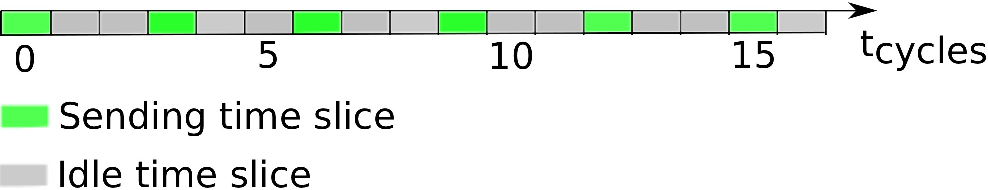
\includegraphics[width=0.8\textwidth]{Chapter3/figures/MAC.pdf}  
  \caption{Time Slicing Communication.}
  \label{fig:TimeSlicing}
\end{figure} 


\section{Goalkeeper Behavior}
This section presents the behavior that leads goalkeeper to make decisions and choose actions for himself. As we said in Section \ref{Architecture}, goalkeeper is the only agent in our team who ``runs'' his own behavior. His behavior depends on a finite state machine. His initial state is ``\textbf{start}'' state. In this state goalkeeper tries to move himself in the center of his goal. When he accomplishes moving there, we change his FSM's state to ``\textbf{Guard}'' state. In guard state he makes use of the \textbf{Watch Object Movement} action to figure the ball's position and the possible direction and speed of its movement.
\begin{figure}[!h]
\centering
  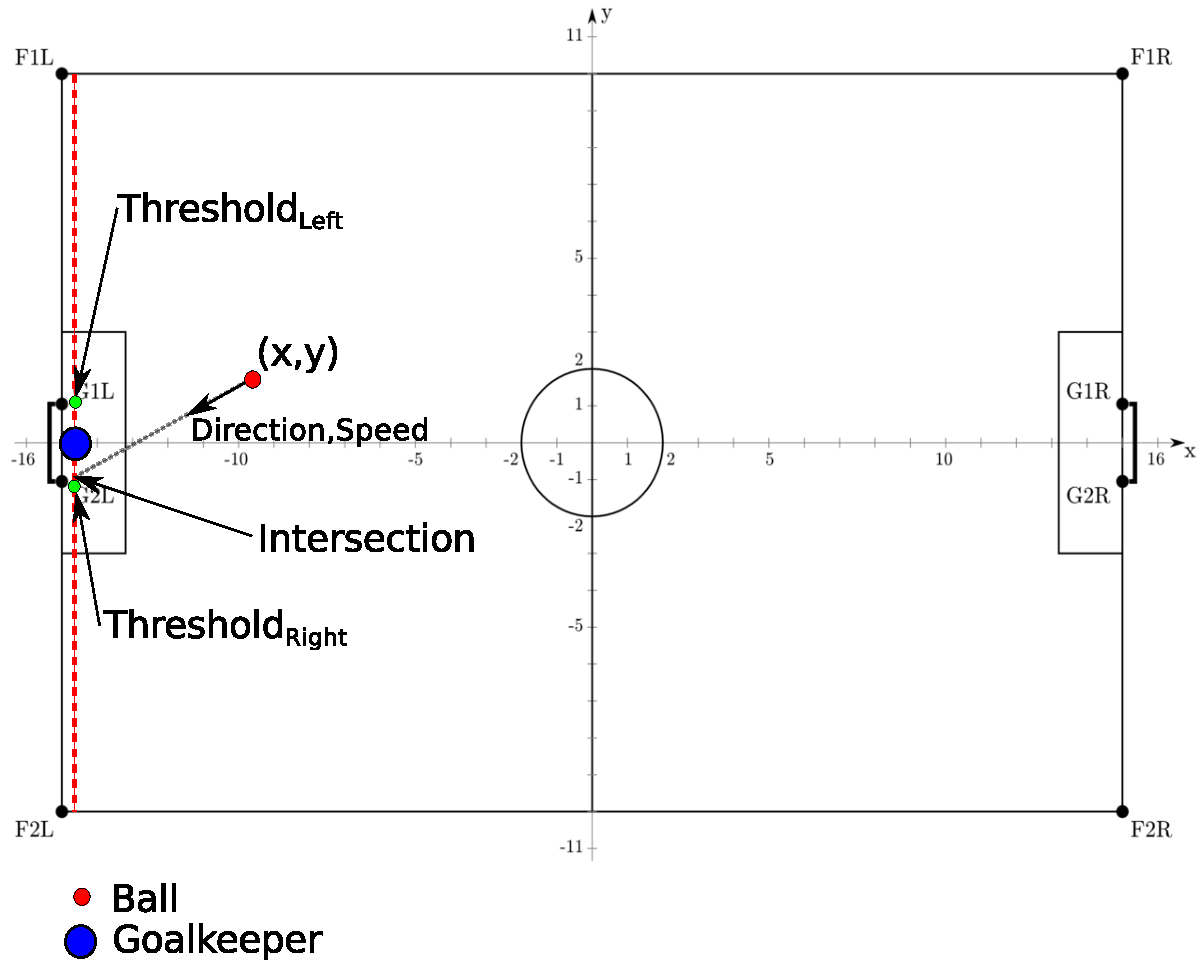
\includegraphics[trim = 0cm 0cm 10cm 0cm, clip,width=0.6\textwidth]{Chapter3/figures/Goalie.pdf}  
  \caption{Goalkeeper Fall Function.}
  \label{fig:Goalkeeper}
\end{figure} 
Figure \ref{fig:Goalkeeper} is going to help you understand easier this state's basic idea. Goalkeeper Considers his position as the start of both axis x and y due to difficulties in making use of the localization process. So, red dashed line determines the goalkeeper's y-axis and x-axis. For every movement of the ball he tries to compute if there is an intersection point between his y-axis and the grey dashed line which starts from ball's position in the direction of ball's movement. If there is an intersection point between these two lines then agents computes if this point is out of the two thresholds ($Threshold_{Right}$,$Threshold_{Left}$). If not, we are pretty sure that ball is heading towards our goal. We compute how much time will take to the ball to meet our y-axis according to its speed and taking account the friction between ball and the ground. If this time is equal or less than the time takes our agent to fall, agent performs a right or a left fall. You can see agent falling to prevent a goal in Figure \ref{fig:GoalkeeperFall}. There are also other states. State ``\textbf{Libero}'' is a state in which goalkeeper sees the ball into his box and there are no other agents near to it. Then goalkeeper goes to clear the ball from his box. Through coordination process informs other field players that he is at ``libero'' state to prevent them from going towards the ball too. When he clears the ball, he returns to his initial position. 

\begin{figure}[!h] 
  \begin{center}
    \subfigure{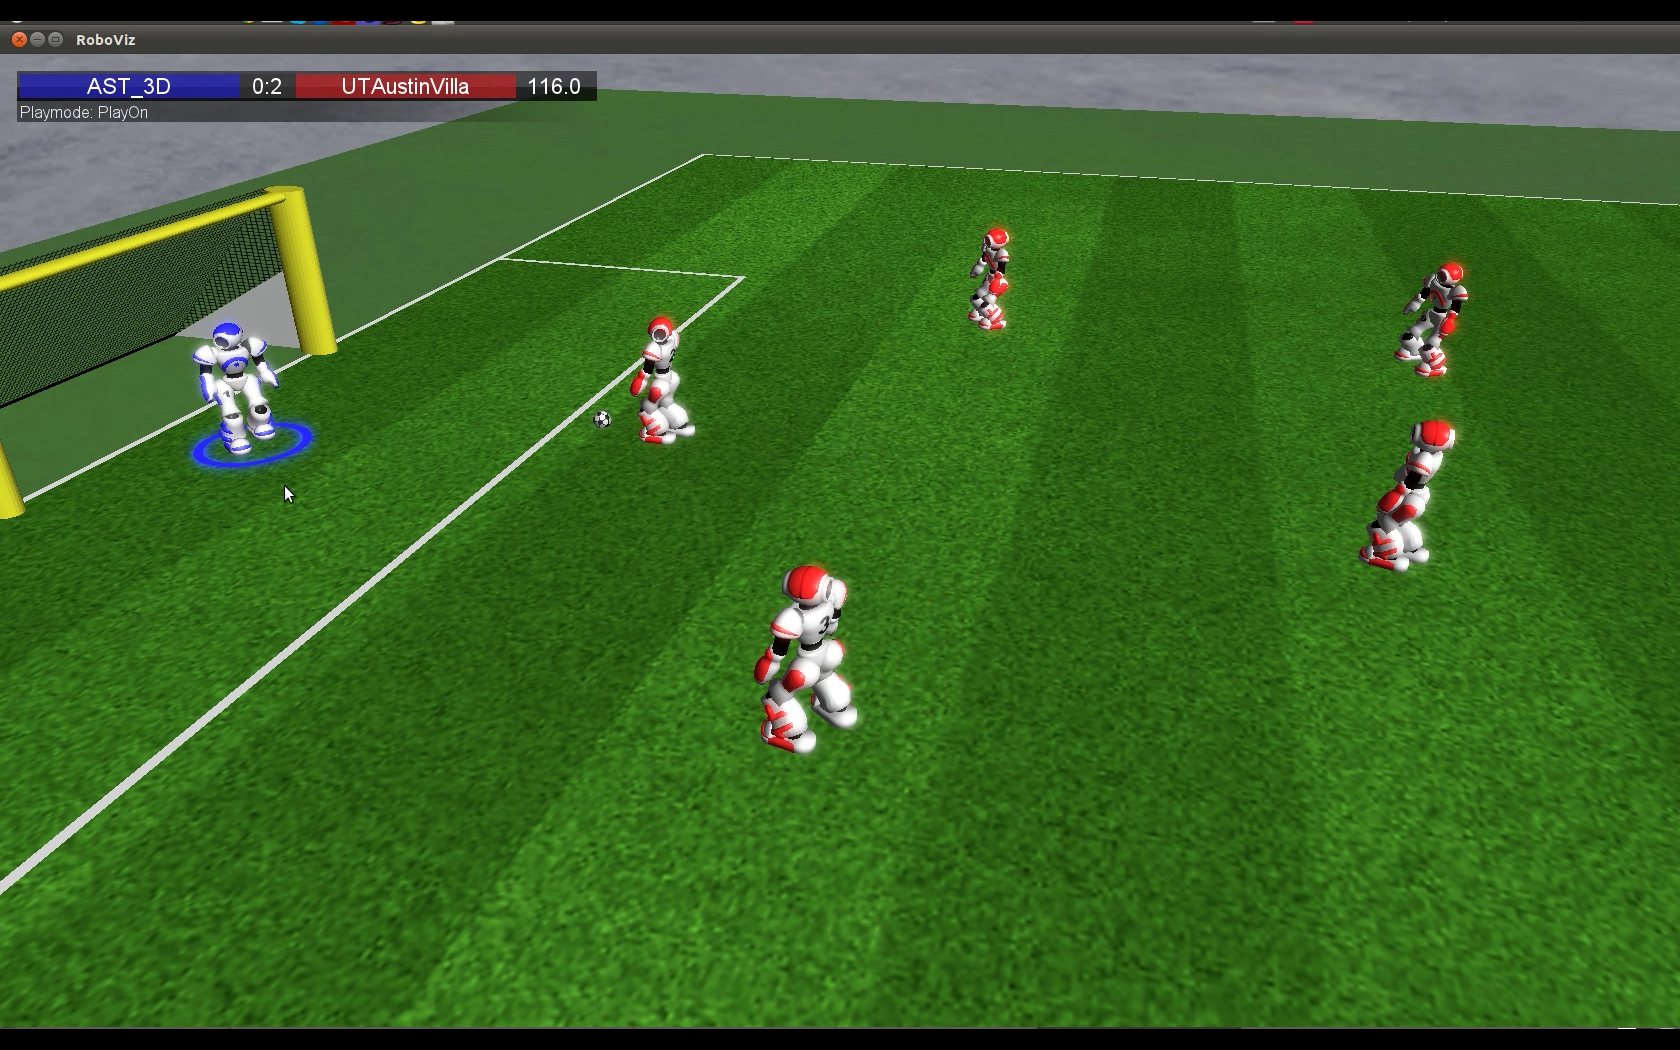
\includegraphics[trim = 5cm 10cm 30cm 5cm, clip,scale=0.25]{Chapter3/figures/GoalieFall.png}}\
    \subfigure{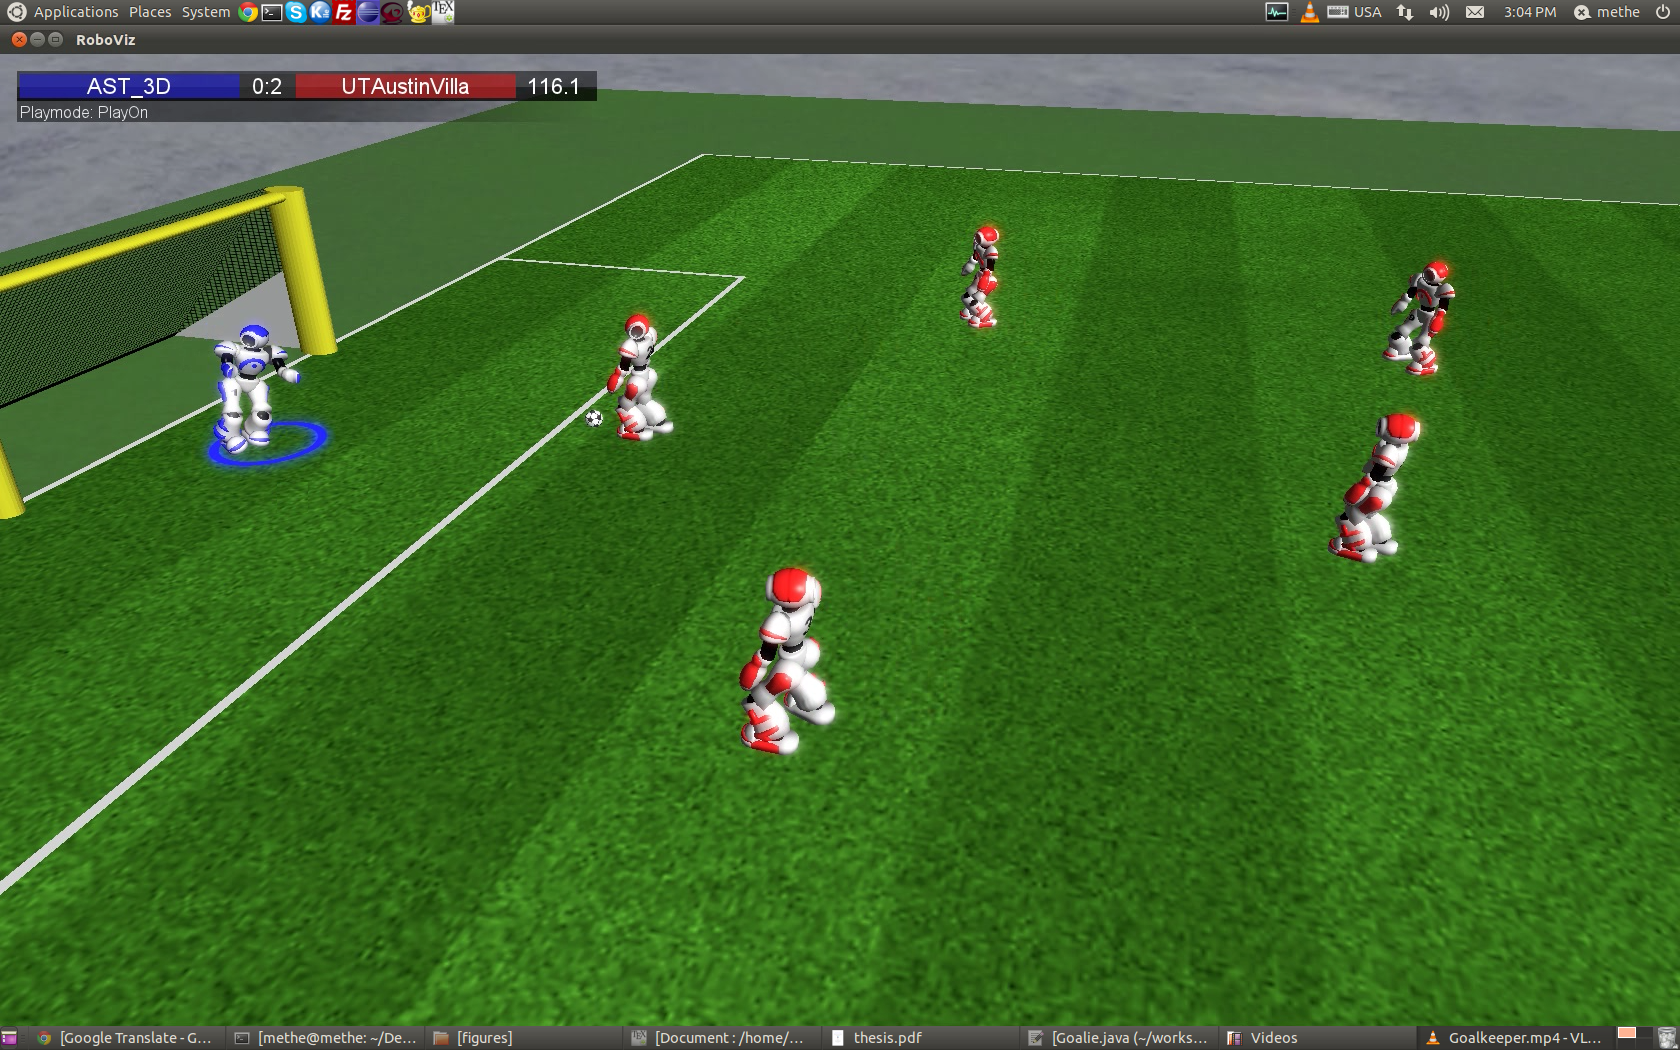
\includegraphics[trim = 5cm 10cm 30cm 5cm, clip,scale=0.25]{Chapter3/figures/GoalieFall2.png}}\\
    \subfigure{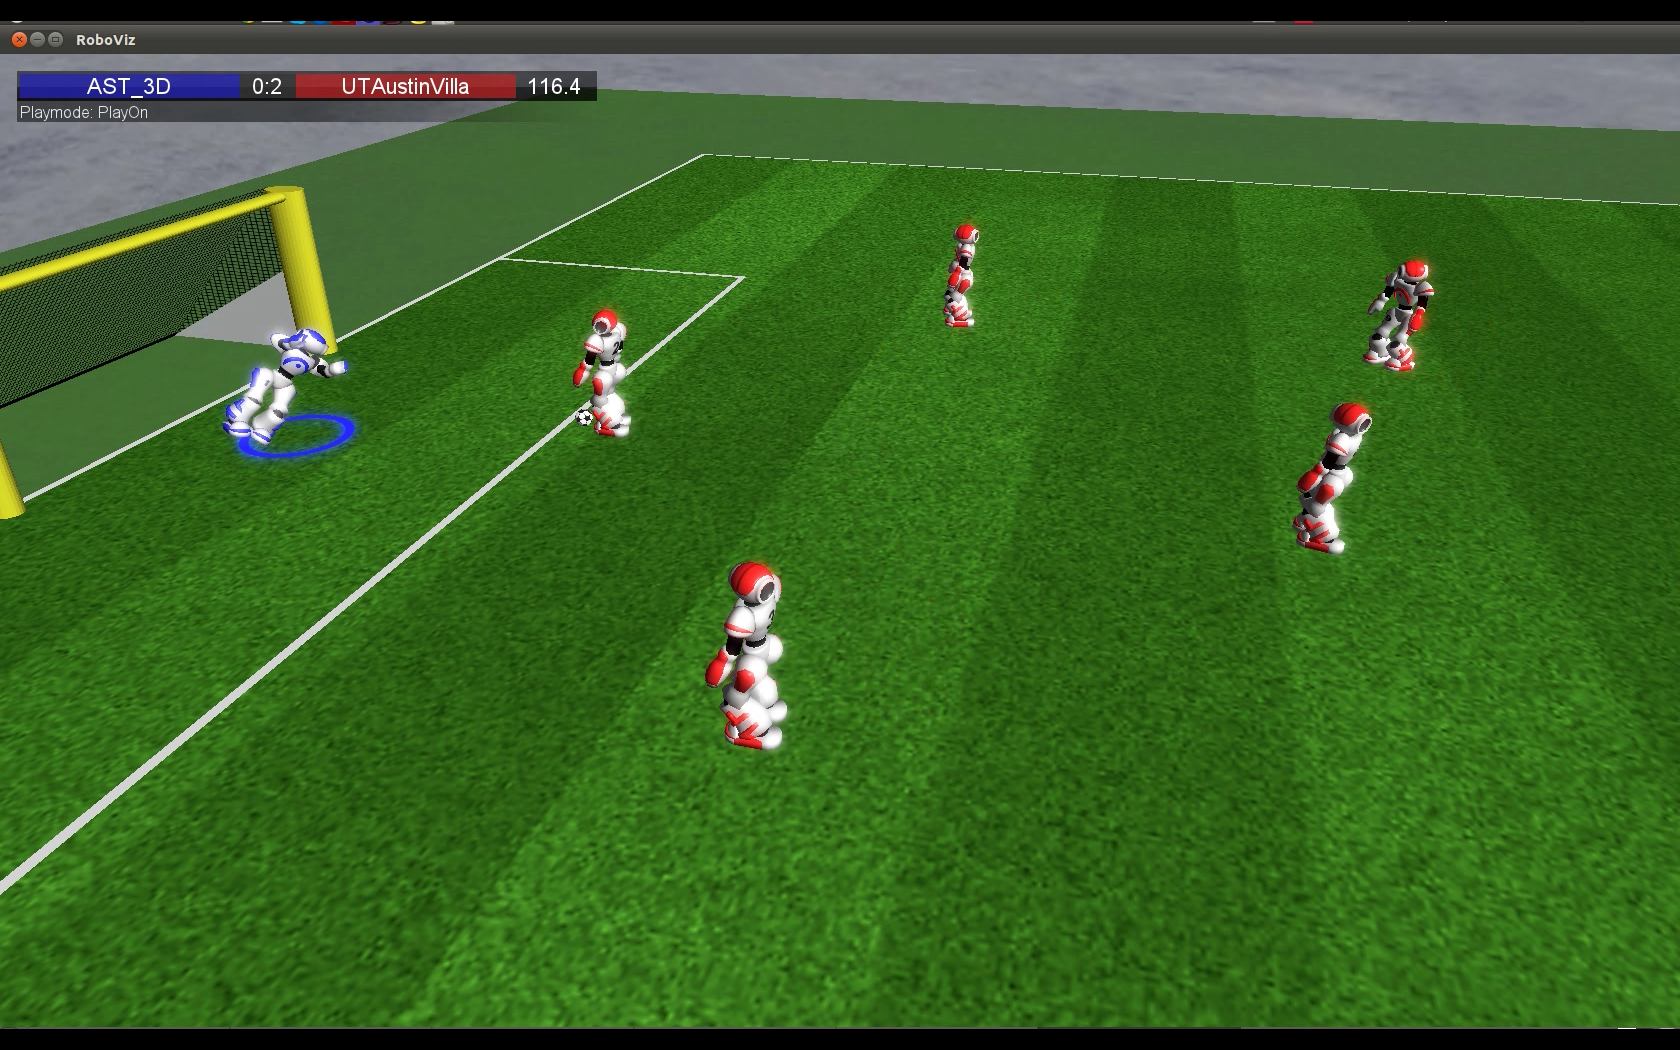
\includegraphics[trim = 5cm 10cm 30cm 5cm, clip,scale=0.25]{Chapter3/figures/GoalieFall3.png}}\
    \subfigure{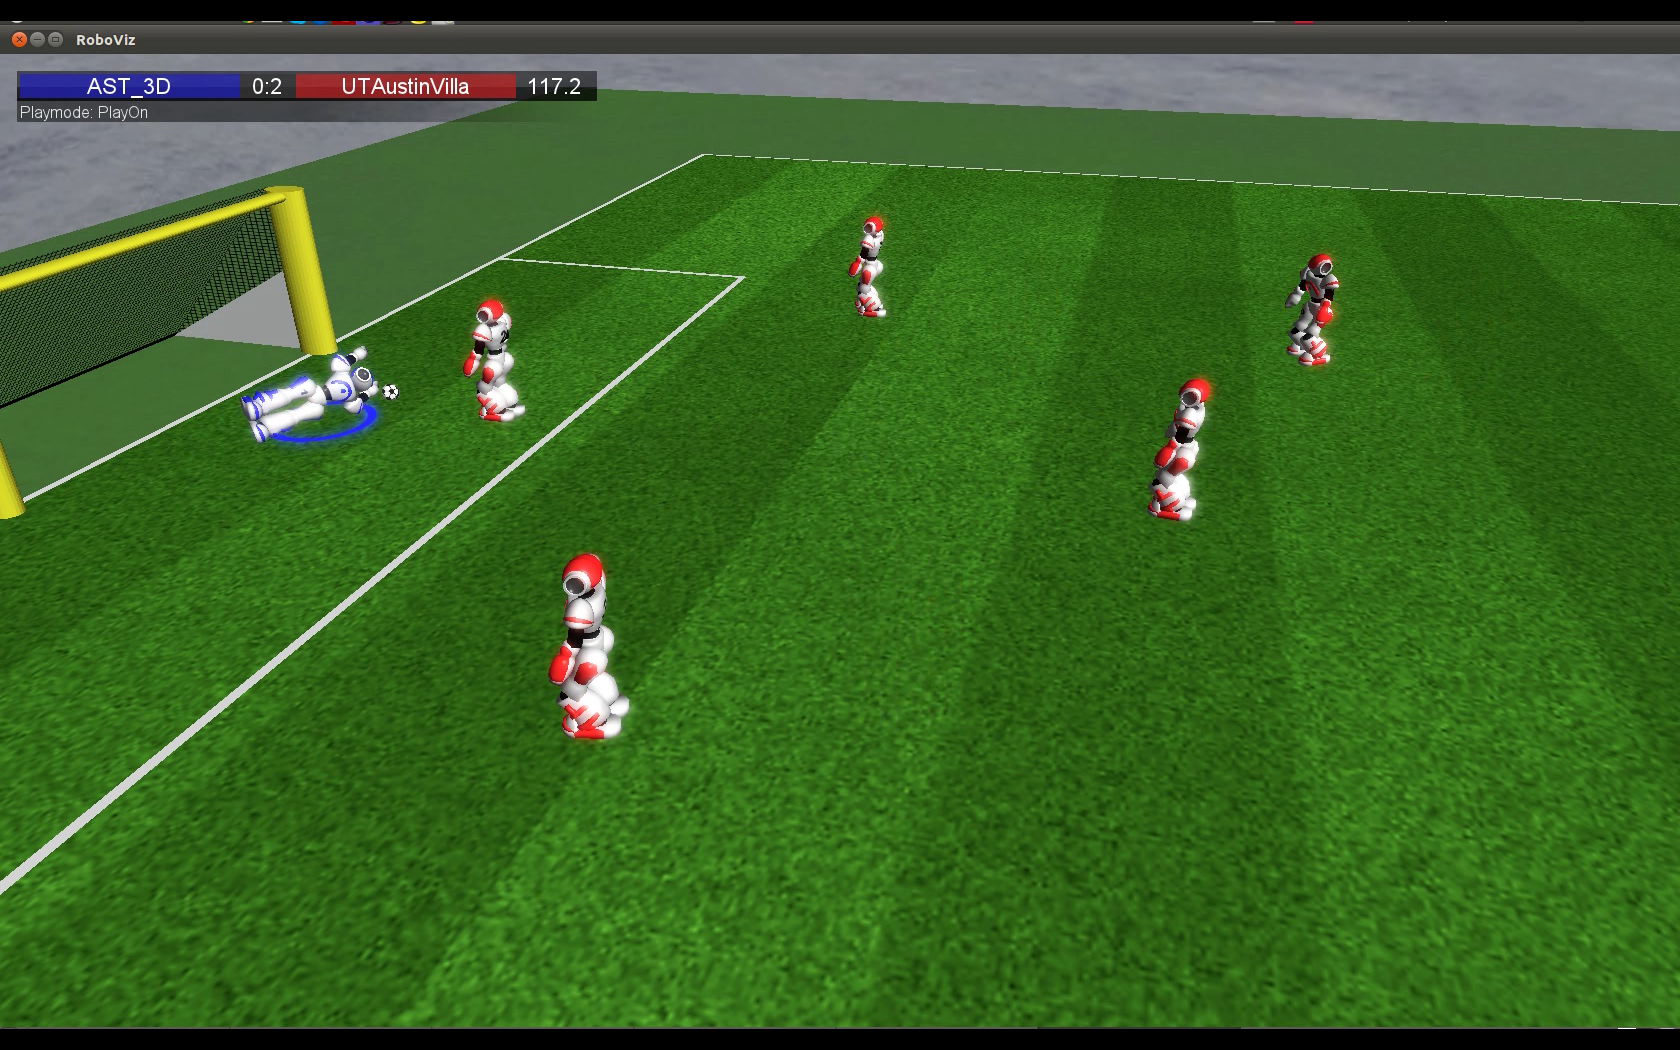
\includegraphics[trim = 5cm 10cm 30cm 5cm, clip,scale=0.25]{Chapter3/figures/GoalieFall4.png}}\
  \end{center}
  \caption{Goalkeeper Falls to Prevent Opponents from Scoring.}
  \label{fig:GoalkeeperFall}
\end{figure}

